%**********************************************************
\section{Tools Setup}
Before doing the system configuration it is necessary to first setup all of the used tools, as will be next presented.

%**********************************************************
\subsection{Git}
In order to make collaboration easier, allowing change by multiple people to all be merged into one source, Git will be used. Git is the most commonly used version control system. Before using it, it is necessary to do the correct setup as shown bellow.
\begin{lstlisting}
$ sudo apt install git
$ git config --global user.name "John Doe"
$ git config --global user.email johndoe@example.com
$ git config --global core.editor subl
$ cd ~
$ git clone git@github.com:ESRGgroup9/slipad.git
\end{lstlisting}

With this steps, Git is installed in a local machine, username and user email is defined alongside with the default core editor. After this, one can clone the repository for this project, created in GitHub, by executing line 6.

%**********************************************************
\subsection{Buildroot}
Buildroot is a simple, efficient and easy-to-use tool used to generate this project's embedded Linux system, through cross-compilation. The steps in order to install Buildroot in a local machine is shown bellow.

\begin{lstlisting}
$ cd ~
$ mkdir buildroot
$ cd buildroot
$ wget https://buildroot.org/downloads/buildroot-2021.02.5.tar.gz
$ tar xzf buildroot-2021.02.5.tar.gz
$ cd buildroot-2021.02.5
\end{lstlisting}

After the installation is done, one can do the base configurations, essential to the support the rest of the configurations.
\begin{lstlisting}
$ make raspberrypi4_defconfig
$ make menuconfig
$ make xconfig
$ make 
$ make clean
\end{lstlisting}

The first command is used to configure a kernel image for the Raspberry Pi 4, as it does the necessary configurations regarding hardware handling along with fetching some board specific packages. Then with the second and third commands, one can generate the graphic interface seen in figure \ref{fig:menuconfig}, presenting several sub-menus. 

\begin{figure}[H]
	\centering	
	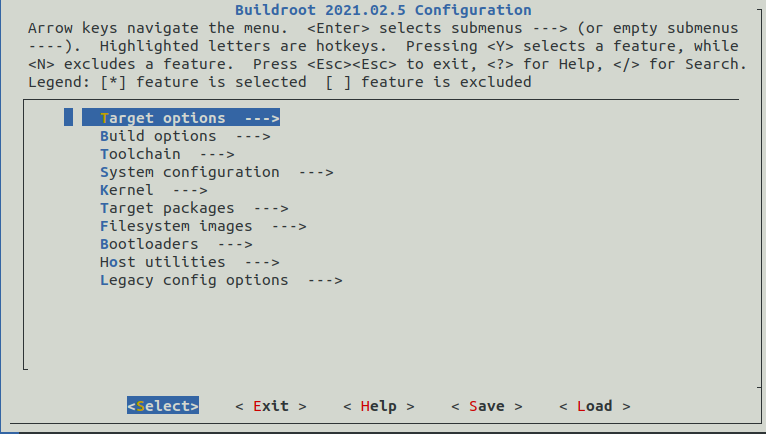
\includegraphics[width=.74\textwidth]{11configs/menuconfig}
	\caption{Buildroot menuconfig.}
	\label{fig:menuconfig}
\end{figure}

%**********************************************************
\subsection{OpenCV}

\begin{lstlisting}
$ cd ~/buildroot/buildroot-2021.02.5/output/build/opencv3-3.4.13/buildroot-build
$ cmake-gui
$ cmake .
$ make -j8
$ sudo make install
\end{lstlisting}

%**********************************************************
\subsection{Qt Creator}

The Qt Creator IDE was used to create an application that is used by the operator to interact with the system. The IDE instalation is done by downloading the open-source online installer present on the official site, in the download page \cite{qt_creator}. In the figure \ref{fig:qt_instalation} is shown all the packages installed for this IDE.

\begin{figure}[H]
	\centering	
	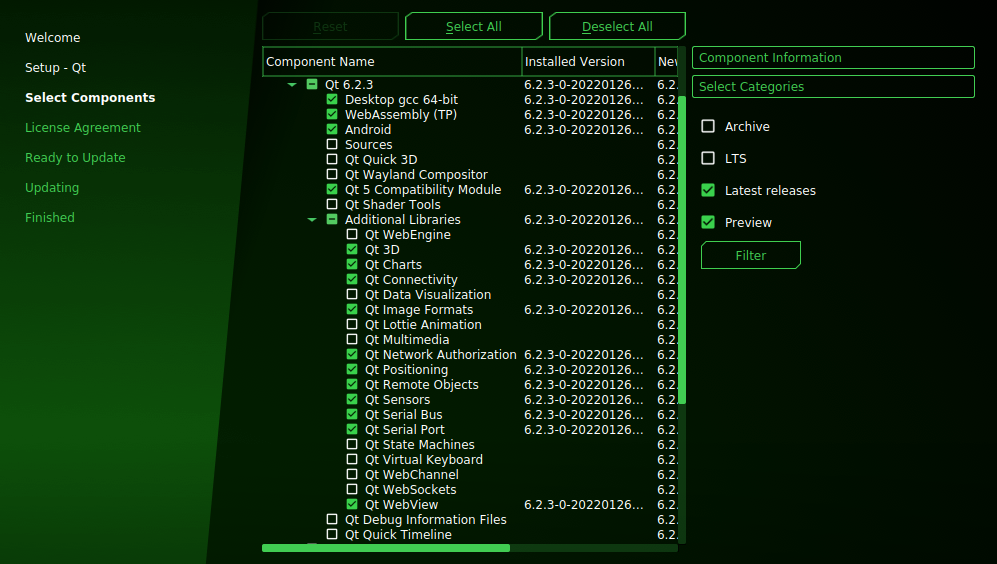
\includegraphics[width=.80\textwidth]{11configs/qt_instalation}
	\caption{Qt Creator: Instalation.}
	\label{fig:qt_instalation}
\end{figure}

Since one is deploying the application to an Android device, it was necessary to install and configure the Android Studio and SDK tools \cite{android_studio}, and also Android NDK \cite{android_ndk} in the Qt Creator. To install the Android Studio run \verb|<path-to-android-studio>/android-studio/bin/studio.sh|. Next, one needs to configure the platform of the Android Studio accordingly to the android phone version. The Android NDK must be the \verb|r23| version, and the Qt creator configure the packages missing.

It is also necessary to install a Java SE Development (JDK) \cite{java}. The JDK version shouldn't be the latest and the installed one was the version 11. Now, run \verb|<path-to-android-studio>/android/tools/bin/sdkmanager --licenses| in order to accept the licenses. 

At last, the \verb|QT -> Tools -> Options -> Devices -> Android|, sould look like shown in figure \ref{fig:qt_config}.

\begin{figure}[H]
	\centering	
	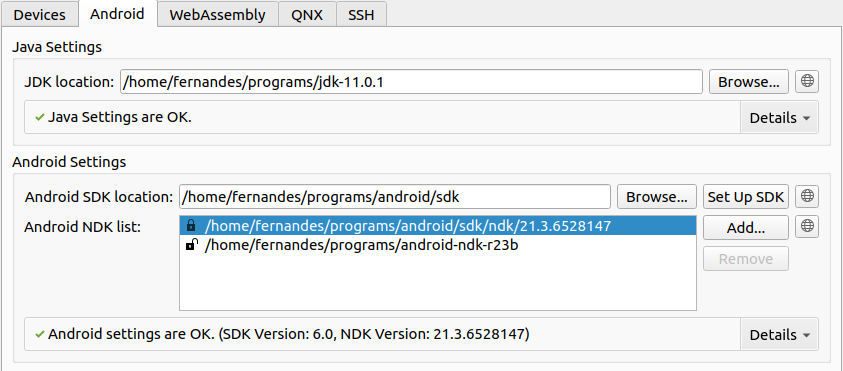
\includegraphics[width=.80\textwidth]{11configs/qt_config}
	\caption{Qt Creator: Configuration.}
	\label{fig:qt_config}
\end{figure}

%**********************************************************
\subsection{MySQL}
In order to have a fully managed database service to deploy cloud-native applications as MySQL, one has to firstly install it properly, as shown bellow.

\begin{lstlisting}
$ sudo apt-get install libmysqlclient-dev
\end{lstlisting}

First time runnning \verb|mysql|, one can create a strong password for \verb|mysql| access. After that, one can login into \verb|mysql| by typing:

\begin{lstlisting}
$ mysql -u root -p
\end{lstlisting}

%**********************************************************
\subsection{PHP}
In order to fetch data from the remote server database to the website that will present available parking spots, one uses PHP, which must first be configured. The following commands must be executed so that one gets a PHP client and PHP with MySql.

\begin{lstlisting}
$ sudo apt install php7.4-cli
$ sudo apt install php-mysqli
\end{lstlisting}

Knowing that fetching data from a remote database envolves secret keys, such as servername, username, port number, database password, it is usefull to have a \verb|.env| file which will contain all of them. In order to load those variables into the website index file one needs to setup \verb|phpdotenv| following the steps bellow. \cite{phpdotenv}

\begin{lstlisting}
$ sudo apt install composer
$ composer install
$ composer require vlucas/phpdotenv
\end{lstlisting}

%**********************************************************
\subsection{Google Maps Credentials}
In order for the website to present the parking spaces at a given location in a map, one uses Google Maps API. In order to generate a Google API key, one needs to go to Google API Console \cite{googleapi} and:

\begin{enumerate}
	\item Create a \textbf{new project};
	\item In API Manager go into \textbf{Library} and select \textbf{Google Maps Javascript API};
	\item Select the created project to enable APIs;
	\item Enable API;
	\item In API Manager go into \textbf{Credentials} and in \textbf{Create Credentials} click \textbf{Create API key}	
\end{enumerate}

After this steps, one may retrieve the generated key and use it within website source file. Make sure that this does not leak since it is a secret key that it is not meant be shared.

%**********************************************************
\clearpage
\section{System Configuration}
\label{systemConfig}

In the Buildroot, using \verb|make menuconfig| one can use a graphic interface (as previously shown in figure \ref{fig:menuconfig}) to select packages and change configurations in order to create a custom linux image.\\

Under \verb|Target-Packages| select:
\begin{itemize}
%	\item \verb|Development tools|, select:
%	\begin{itemize}
%		\item \verb|git|
%	\end{itemize}
	
	% *****************************************************************************
	\item \verb|Networking applications|, select:
	\begin{itemize}
		\item \verb|arp-scan|: scan the network of a certain interface for alive hosts;
		\item \verb|arptables-legacy|: set up and maintain the tables of ARP rules;
		\item \verb|dhcpcd|: open source DHCP client;
		\item \verb|dropbear|: small SSH server which will let us log in remotely;
	\end{itemize}
	
	% *****************************************************************************
	\item \verb|Hardware Handling|
	\begin{itemize}
		\item \verb|spi-tools|: tools needed to use SPI. Used for LoRa module communication;
		\item \verb|i2c-tools|: tools needed to use I2C. Used for light sensor module, TSL2581;
		\item \verb|rpi-userland|: Used to detect camera hardware;
	\end{itemize}
	
	% *****************************************************************************
	\item \verb|Libraries|, select:
	\begin{itemize}
		% *******************************
		\item \verb|Hardware Handling|
		\begin{itemize}
			\item \verb|bcm2835|: C library for Raspberry Pi user programs;
			\item \verb|libv4l|: select \verb|v4l-utils tools|: API for real time video capture;
		\end{itemize}
		
		% *******************************
		\item \verb|Graphics|
		\begin{itemize}
			\item \verb|OpenCV3|: select \verb|jpeg support|, \verb|png support|, \verb|v4L support|, \verb|videoio|, \verb|highgui|, \verb|imgcodecs|, \verb|imgproc|, \verb|v4l support|: Used for image capturing and processing;
		\end{itemize}
	\end{itemize}

	% *****************************************************************************
	\item \verb|Audio and Video Applications|, select:
	\begin{itemize}
		\item \verb|v4l2grab|: utility for grabbing JPEG images;
	\end{itemize}
	% *****************************************************************************
	
\end{itemize}

%**********************************************************
\clearpage
\section{Image Generation}
After all the necessary tools, packages and configurations are done, one needs to finally create the Linux custom image, that will run on the Raspberry Pi.

\begin{lstlisting}
$ cd ~/buildroot/buildroot-2021.02.5/
$ make
\end{lstlisting}

After that one can copy the image into the SD card, that will go into the Raspberry Pi. For that one can use the linux \verb|dd| command. \cite{dd}

\begin{lstlisting}
$ sudo dd if=./output/images/sdcard.img of=/dev/sdb
\end{lstlisting}

With this command, one must define the input file, \verb|if|, which is the linux image, and the output file, \verb|of|, which is the SD card, being in this example named \verb|sdb|.


%**********************************************************
%\clearpage
\section{System Initialization}
The Buildroot generates the boot configuration, in the \verb|/boot/config.txt| file that contains system configuration parameters that are read when the system boots from the microSD card, and that would traditionally be edited and stored using a BIOS. \cite{configtxt} The listing \ref{lst:configtxt} shows the boot configuration file. For this project, one added the parameter in line 24, in order to enable the I2C device, the parameters in lines 26 and 27, to activate the camera.

\begin{lstlisting}[caption={/boot/config.txt file.}, label={lst:configtxt}]
# We always use the same names, the real used variant is selected by
# BR2_PACKAGE_RPI_FIRMWARE_{DEFAULT,X,CD} choice
start_file=start.elf
fixup_file=fixup.dat

kernel=zImage

# To use an external initramfs file
#initramfs rootfs.cpio.gz

# Disable overscan assuming the display supports displaying the full resolution
# If the text shown on the screen disappears off the edge, comment this out
disable_overscan=1

# How much memory in MB to assign to the GPU on Pi models having
# 256, 512 or 1024 MB total memory
gpu_mem_256=100
gpu_mem_512=100
gpu_mem_1024=100

# fixes rpi (3B, 3B+, 3A+, 4B and Zero W) ttyAMA0 serial console
dtoverlay=miniuart-bt

dtparam=i2c_arm=on 		# enable i2c

start_x=1             	# enable camera
gpu_mem=128           
\end{lstlisting}

%**********************************************************
\subsection{Init Scripts}
\verb|/etc/init.d| is a directory containing initialization and termination scripts for changing init states. File names in this directory are of the form \verb|[SK]nn<init.d filename>|, where \verb|S| means start this job, \verb|K| means kill this job, and \verb|nn| is the relative sequence number for killing or starting the job. \cite{initScript} For this reason, one must create a script, with name started by \verb|S|, inside \verb|/etc/init.d| in the Raspberry Pi, using for that, \verb|vi|.

In order to guarantee that each program is running after the system boots up, its necessary to create the respective init scripts, following the procedure detailed in listing \ref{lst:initScript}.

\begin{lstlisting}[caption={Procedure for creating an init script, named Sscript\_name}, label={lst:initScript}]
$ cd /etc/init.d
$ vi S<scriptName>.sh
$ chmod +x S<scriptName>.sh
\end{lstlisting}

The local system has the init script detailed bellow, in listing \ref{lst:lsScript}. This script must insert all necessary device drivers in order to correctly execute the local system's daemon, dSensors, and the main process. 

\begin{lstlisting}[caption={Init script for local system.}, label={lst:lsScript}]
#!/bin/sh

# Inserting i2c-tools
modprobe i2c-bcm2835
modprobe i2c-dev

# Inserting PIR DDriver
insmod /etc/pir.ko

# Inserting lampf DDriver
insmod /etc/lampf.ko

# Run local system's daemon sensor and main process
/etc/dSensors.elf &
/etc/localSys.elf
\end{lstlisting}

The gateway system has the init script detailed in listing \ref{lst:gatScript}. The gateway, \verb|gateway.elf| is connected via TCP-IP to the remote system. Therefore one can set the gateway to connect to \verb|10.42.0.1|, which is the network address of remote system in the same network as the gateway, in port \verb|5000|.

\begin{lstlisting}[caption={Init script for Gateway system.}, label={lst:gatScript}]
#!/bin/sh

etc/gateway.elf 10.42.0.1 5000
\end{lstlisting}

The remote system also has an init script, as shown in listing \ref{lst:rsScript}. This is responsible for running the website PHP server \cite{phpserver} and running the remote system in port \verb|5000|.

\begin{lstlisting}[caption={Init script for remote system.}, label={lst:rsScript}]
#!/bin/sh

# run website PHP server
php -S localhost:8000 -t ~/slipad/remoteSystem/website/ &

# run remote system
~/slipad/remoteSystem/bin/remoteSystem.elf 5000

\end{lstlisting}

%**********************************************************
\clearpage
\section{Device Drivers}
\subsection{tsl2581}
%.config - Linux/arm 5.10.1 Kernel Configuration
%> Device Drivers > Industrial I/O support > Light sensors
%
%-> TAOS TSL2580, TSL2581 and TSL2583 light-to-digital converters
%
%cat /lib/modules/5.10.1-v7l/modules.dep | grep tsl
In order to insert the \verb|tsl2581| device driver, available on the Linux kernel (\cite{code_tsl}) one needs to execute a series of steps.\\

Firstly, one needs to add a new entry on the Raspberry Pi device tree, regarding the \verb|tsl2581|. For that, one needs to change the Device tree Source file (.dts) for the Raspberry Pi, named \verb|bcm2711-rpi-4-b.dts|. This will be later compiled into a device tree binary (.dtb), when creating an image using Buildroot, which will be later passed by the boot loader to the operating system kernel. \cite{dtb}

\begin{lstlisting}
$ cd ~/buildroot/buildroot-2021.02.5/output/build/linux-custom/arch/arm/boot/dts
$ nano bcm2711-rpi-4-b.dts
\end{lstlisting}

At the end of the file, before \verb|__overrrides__|, the following code must be added, where \verb|reg| is the I2C address of the device. \cite{tsl2583_txt} 

\begin{lstlisting}
&i2c1 {
	status = "okay";
	
	tsl2581@29 {
		compatible = "amstaos,tsl2581";
		reg = <0x29>;
	};
};
\end{lstlisting}

For the Raspberry Pi, in the \verb|/boot/config.txt| file, one must enable \verb|i2c1| with a \verb|dtoverlay|, by adding the line of code shown next.
\begin{lstlisting}
dtoverlay=i2c1
\end{lstlisting}

When booting the Raspberry Pi, one must insert the \verb|tsl2581| device driver, but before that, some modules must be added using \verb|modprobe|.

This is an I2C based sensor, which uses the \ac{iio} interface. In order to provide the \ac{iio} API, needed in the device driver to be used, it is necessary to enable the \ac{iio} kernel subsystem, \verb|industrialio|. To enable the I2C bus, one must load the \verb|i2c-bcm2835| module. \cite{i2c_bcm2835}\\

After that, one can insert the \verb|tsl2581| device driver, \verb|ldr.ko|.

\begin{lstlisting}
$ modprobe industrialio
$ modprobe i2c-bcm2835
$ insmod ldr.ko
\end{lstlisting}

After the device driver insertion, one can use it to communicate with the sensor in order to acquire the ambient luminosity. For that, a “single” on-demand read can be issued by user-space directly by reading \linebreak \verb|/sys/bus/devices/iio:device/in_<type><index>_raw|. In this case, the \verb|read_raw()| callback should handle basically all the steps necessary to get the required measurement. \cite{read_tsl}
%**********************************************************
\subsection{PIR}

%**********************************************************
\clearpage
\section{LoRa communication}
LoRa communication was implemented by deriving a third-party software from Arduino. \cite{sx1278_lib} Using \verb|bcm2835| C library one was able to control all the needed GPIO and SPI functions. \cite{bcm2835}

By reading the LoRa module SX1278 documentation \cite{sx1278}, one is able to find the figure \ref{fig:sx1278_spi}. The SPI interface gives access to the configuration register via a synchronous full-duplex protocol. One of three access modes to the registers is used - SINGLE access. In this mode:
\begin{itemize}
	\item \textbf{Write access:} an address byte followed by a data byte is sent;
	\item \textbf{Read access:} an address byte is sent and a read byte is received;
\end{itemize}

\begin{figure}[H]
	\centering	
	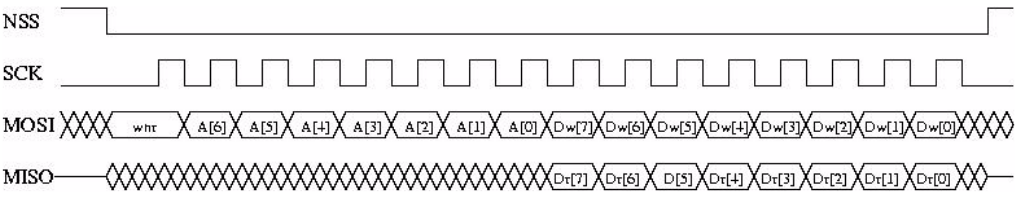
\includegraphics[width=1\textwidth]{12implementation/sx1278_spi}
	\caption{SPI Timing Diagram (single access).}
	\label{fig:sx1278_spi}
\end{figure}

A transfer is always started by the NSS pin going low. MISO is high impedance when NSS is high. MOSI is generated by the master on the falling edge of SCK and is sampled by the slave on the rising edge of SCK. MISO is generated by the slave on the falling edge of SCK.

A LoRa message is defined by the class \verb|LoRaMsg| having the attributes shown in listing \ref{lst:loramsg}.

\begin{lstlisting}[caption={LoRa message}, label={lst:loramsg}]
int recvAddr;     	// receiver address
int sendAddr;     	// sender address

int msgID;        	// message ID
size_t msgLength; 	// message length
string msg;       	// message
\end{lstlisting}


